\subsubsection{TAPER}

TAPER (query-aware, partition-enhancement for large, heterogeneous, graphs) \cite{Taper} --- система предложенная Хьюго Фертом и Паоло Миссье. Данное решение представляет собой фреймворк для инкрементального улучшения существующих распределений графов, используя специальную структуру TPSTrie.

\textit{Экстраверсия и интроверсия вершин}

Для количественной оценки вклада каждой вершины в межшардовые переходы вводятся понятия интроверсии и экстраверсии. Эти показатели базируются на вероятностной модели обхода графа, учитывающей паттерны запросов.

\begin{figure}[h]
    \centering
    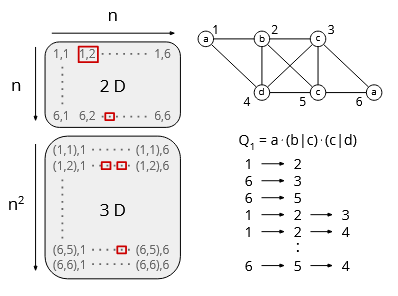
\includegraphics[width=0.6\textwidth]{extras/taper/visitor_matrix.png}
    \caption{Структура Visitor Matrix (VM) для хранения вероятностей путей различной длины}
    \label{taper-fig:vm_structure}
\end{figure}

Пусть задан путь $p = v_{i_1} \rightarrow \ldots \rightarrow v_{i_k} \rightarrow v$, соответствующий одному из паттернов запросов. Вероятность этого пути $Pr(p)$ может быть вычислена как произведение условных вероятностей переходов. Интроверсия вершины $v \in V_i$ (где $V_i$~--- её родной шард) определяется как суммарная вероятность всех путей, ведущих к $v$, при условии, что следующий шаг также остаётся внутри $V_i$:
$$
\text{introversion}(v) = \frac{1}{Pr(v)} \sum_{p \in \text{paths}(v,V_i)} \left( Pr(p) \cdot \sum_{v' \in V_i} VM_i(t)[p, v'] \right),
$$
где $VM_i(t)$ --- матрица посещений (Visitor Matrix), структура которой показана на рисунке \ref{taper-fig:vm_structure}, для шарда $i$, хранящая вероятности переходов для путей длины до $t$, а $Pr(v)$ --- нормировочный коэффициент (суммарная вероятность всех путей, ведущих к $v$). Экстраверсия, соответственно, является дополнением до единицы:
$$
\text{extroversion}(v) = 1 - \text{introversion}(v).
$$
Именно экстраверсия служит для TAPER сигналом к перемещению вершины.

\textit{Представление нагрузки запросов: TPSTrie}

Прямое вычисление VM имеет экспоненциальную сложность $O(|V|^t)$ и неприменимо для больших графов. Для решения этой проблемы предлагается компактная структуру данных --- префиксное дерево обобщения паттернов обхода (Traversal Pattern Summary Trie, TPSTrie),. Идея заключается в том, чтобы хранить не вероятности для конкретных вершин, а вероятности для последовательностей меток, которые требуются в запросах. Построение TPSTrie показано на рисунке \ref{taper-fig:tpstrie_construction}.

\begin{figure}[ht]
    \centering
    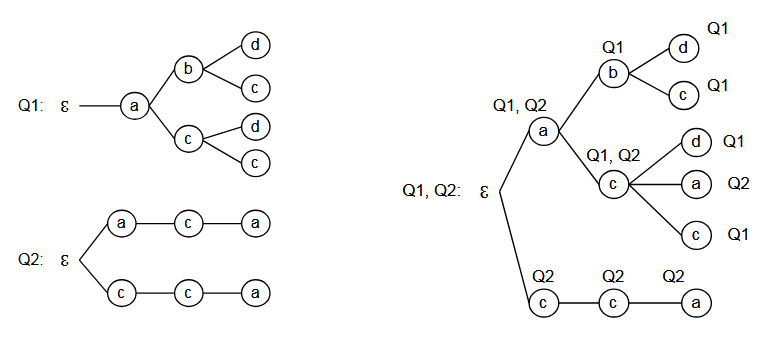
\includegraphics[width=\textwidth]{extras/taper/tree_construction.png}
    \caption{Построение TPSTrie путём разбора регулярных выражений запросов и объединения результатов}
    \label{taper-fig:tpstrie_construction}
\end{figure}

Каждый узел TPSTrie соответствует некоторой последовательности меток и помечается множеством запросов, которые могут породить такую последовательность. Каждому узлу ставится в соответствие вероятность $p(n)$, вычисляемая на основе частот запросов и структуры дерева. Например, для корневого перехода $\mathcal{E} \rightarrow a$ вероятность равна:
$$
Pr(\mathcal{E} \rightarrow a) = \sum_{Q_i \in \mathcal{Q}} Pr(\mathcal{E} \rightarrow a | Q_i) \cdot Pr(Q_i),
$$
где условные вероятности определяются количеством возможных первых шагов в запросе $Q_i$. При изменении частот запросов вероятности в узлах дерева пересчитываются, что позволяет TPSTrie адаптироваться к динамике нагрузки.

\textit{От TPSTrie к Visitor Matrix}

Для получения вероятностей переходов между конкретными вершинами (т.е. заполнения VM) используется следующий подход. Для текущей вершины $v_k$ и истории пути $p$ выполняется поиск соответствующего узла в TPSTrie. Полученный узел указывает, какие метки допустимы для следующего шага, и с какими вероятностями. Затем эти вероятности равномерно распределяются среди всех соседей вершины $v_k$, имеющих данную метку. Это даёт вектор вероятностей перехода к каждому соседу, который и является строкой VM. Такой подход позволяет избежать хранения вероятностей для всех возможных путей, заменяя их компактным представлением на уровне меток.

Для дальнейшего снижения вычислительной и пространственной сложности авторы вводят эвристики:
\begin{itemize}
    \item вершины, у которых нет внешних соседей, автоматически считаются безопасными (introversion = 1) и исключаются из рассмотрения;
    \item вычисление экстраверсии вершины прекращается досрочно, если её накопленное значение интроверсии превышает заданный порог безопасности.
\end{itemize}
Это позволяет сосредоточить ресурсы только на наиболее проблемных вершинах.

\textit{Алгоритм уточнения распределения}

Процесс уточнения распределения в TAPER является итеративным и основан на жадном алгоритме рефининга, схожем с Кернигана-Лина/Феддучи-Маттея (Kernighan-Lin / Fiduccia-Mattheyses), но с использованием экстраверсии в качестве целевой функции. Одна итерация (вызов TAPER) состоит из нескольких внутренних шагов, на каждом из которых выполняются следующие действия:

\begin{enumerate}
    \item для каждого шарда строится очередь кандидатов --- вершин с наибольшей экстраверсией;
    \item для вершины-кандидата $v$ определяется её семья (family). Это множество вершин, которые с высокой вероятностью участвуют в тех же путях, что и $v$ (т.е. являются источниками путей к $v$ с вероятностью выше 0.5). Перемещение всей семьи вместе с кандидатом повышает эффективность обмена;
    \item для семьи вычисляется предпочтительный целевой шард $V_j$ (как правило, тот, где находится большинство соседей, участвующих в общих путях);
    \item происходит двухсторонний обмен (offer/receive), проиллюстрированный на рисунке \ref{taper-fig:offer-recieve}:
        \begin{enumerate}
            \item исходный шард оценивает потерю интроверсии при удалении семьи;
            \item целевой шард оценивает потенциальный выигрыш в интроверсии от добавления семьи;
            \item если выигрыш целевой шард превышает потерю исходной, обмен считается кооперативным и выполняется.
        \end{enumerate}
    \item если обмен отклонён, кандидату предлагаются другие соседние шарды в порядке убывания предпочтительности.
\end{enumerate}

\begin{figure}[h]
    \centering
    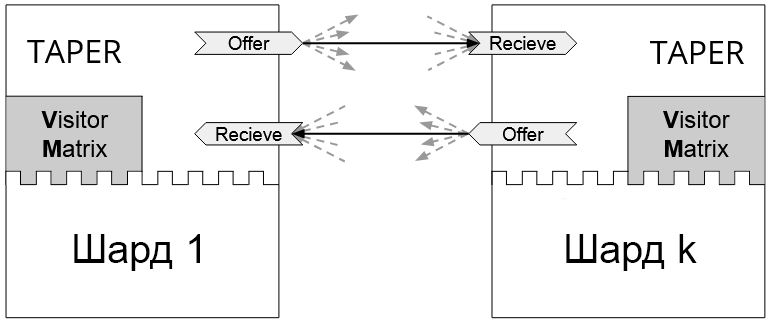
\includegraphics[width=\textwidth]{extras/taper/offer_recieve.png}
    \caption{Схема кооперативного обмена вершинами между шардами}
    \label{taper-fig:offer-recieve}
\end{figure}

Каждая вершина может быть перемещена не более одного раза за внутреннюю итерацию. После обработки всех кандидатов запускается следующая внутренняя итерация. Процесс повторяется до тех пор, пока не будет достигнуто целевое улучшение или максимальное число итераций, при этом строго контролируется баланс размеров шардов (допустимое отклонение, например, 5\%).
